\section{Aufbau von M$^2$etis}
\label{chap:grundlagen:aufbau_metis}

Dieser Abschnitt erläutert den Aufbau von \ac{m2etis} \cite{Fischer2010a, Fischer2010Event} und zeigt den Rahmen dieser Diplomarbeit auf. 

\begin{figure}[htbp]
\centering
\resizebox{\textwidth}{!}{%
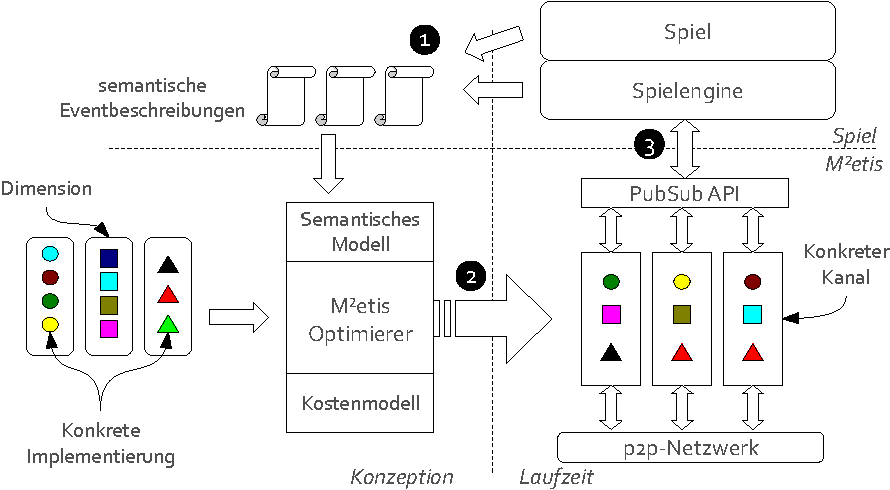
\includegraphics{grafics/metis_aufbau.pdf}}
\caption{Architekturübersicht von \ac{m2etis}}
\label{fig:metis_aufbau}
\end{figure}

\Fref{fig:metis_aufbau} zeigt die Aufteilung des Systemes in \emph{Spiel} und \emph{\ac{m2etis}} sowie die zeitliche Trennung in \emph{Konzeption} und \emph{Laufzeit}.

Im ersten Schritt werden die Eventtypen im Spiel identifiziert und semantisch beschrieben. Auf der linken Seite finden sich beispielhaft verschiedene Dimensionen (nach \cite{Fischer2010a}) sowie deren unterschiedliche Implementierungen. Diese sind dem \emph{\ac{m2etis} Optimierer} bekannt. Dieser verarbeitet im zweiten Schritt unter Zuhilfenahme des \emph{semantischen Modells} und des \emph{Kostenmodells} die semantische Beschreibung der Events und erzeugt für jeden Typ einen optimierten \emph{Kanal}. Wie in der Grafik ersichtlich ist, benötigt das Spiel keine  Implementierungsdetails der einzelnen Kanäle um diese im 3. Schritt zur Laufzeit zu nutzen.

Diese Arbeit ist für die Auswahl des Netzwerkes und die Anbindung an dieses, die Konzeption und prototypische Entwicklung des Publish/Subscribe-Systems zuständig. Damit das Framework einsetzbar ist, werden einige Algorithmen verschiedener Dimensionen implementiert. Die Entwicklung erfolgt als Vorgabe in C++.
